\section{Workflow Abstraction}

\label{sec:abstraction}
The main goal of making an abstraction of a workflow is to be able to reuse it as a whole, or some of its parts, independently of the domain to which they belong to. In this context the concept of classification is crucial because being able to classify a workflow or its parts allows also to index them for easier accesibility. \\

In myExperiment or WINGS the processes of the workflows are not annotated and therefore the abstraction of the different parts of it is not straightforward. Therefore, we have choosen a bottom-up approach in order to study the actual provenance of workflow results (which represents the dataflow) from a set of available workflows at WINGS (@@todo add reference to dataset examples) trying to get some common structures (so called macros) for being able to categorize them and create their taxonomy. The use of the provenance of the workflow results seems to be more appealing that using the workflow templates mainly due to the following two reasons:

\begin{itemize}
\item It actually gathers information from the workflows which really are being used and executed and therefore rewarding the discovery of common patterns of those workflows which really work.
\item It provides the sequence of processes (including their input parameters and their outputs) instead of having the workflow  templates which are represented by acyclic graphs. This allows the dissambiguation of the different possible ways representing a workflow by its actual execution trace (p.e. different possibilities due to "if" control structures).
\end{itemize}

Because of the above mentioned reasons, the provenance of workflow results data is being used for feeding a \textit{trie} structure (@@todo add reference to the code in Github) created to store the different executions of the workflows. This \textit{trie} structure provides the following funcionality:
\begin{itemize}
\item It stores the provenance of the workflow results in an ordered way and the appearance frequency of their processes
\item It calculates relative frecuencies at different levels of the tree
\item It provides different modes to traverse the structure (p.e. preordered)
\item It provides an output XML strcuture with relative frecuencies per level and per process (an output example is available at @@todo include reference).
\end{itemize}

The next picture~\ref{fig:workflowAbstraction} shows the overall discovery process for workflow abstraction. At present we are currently in the second stage which includes the creation of a provenance of workflow results and the \textit{trie} structure explained above. 

\begin{figure}
\begin{center}
\label{fig:workflowAbstraction}
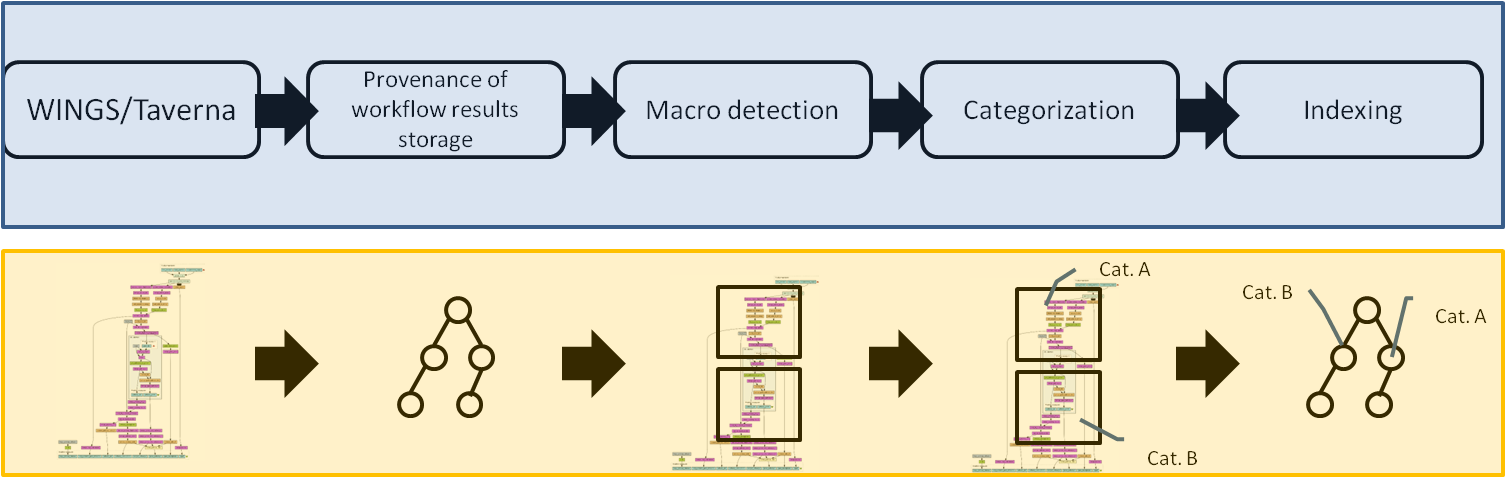
\includegraphics[scale=0.5]{workflowAbstraction}
\caption{Workflow Abstraction Discovery Process}
\end{center}
\end{figure}